\documentclass{article}
\usepackage[pdftex]{graphicx}

\begin{document}

\section{Function visualization}
Sometimes a direct plot of measured data is not the most illuminating way of showing relationships between quantities.  Take for example a (overly) simplified case of trying to understand the relationship between the ``size'' of an object of a particular material and its mass.  For concreteness let's assume our objects are cubes of various sizes, all made of the same unknown metallic material.  We could collect some data on these cubes by measuring the length of a cubes side, $s$, and its mass, $m$.  We might get some data such as follows:

\begin{center}
  \begin{tabular}{ l | r  }
$s$ [cm] & $m$ [g]\\
    \hline
6.49  &	594.68 \\
0.94  &	0.78 \\
6.07  &	469.48 \\
8.24  &	1355.29 \\
3.40  &	123.29 \\
5.47   &	466.92\\
9.11   &	2178.12  \\
1.43   &	22.11   \\
5.22   &	397.79  \\
8.34   &	1605.29 \\
11.01 &	3811.89  \\
8.21   &	1130.73 \\
  \end{tabular}
\end{center}

which we could plot as shown in Figure~\ref{fig:mvss}.  Clearly the data is not linear, $m = As + B$, but it is difficult to tell from this plot what the dependence is.  Even if we assume it is a power law, $m = As^n$, it is hard to look at this and determine what $n$ is.

\begin{figure}
\begin{centering}
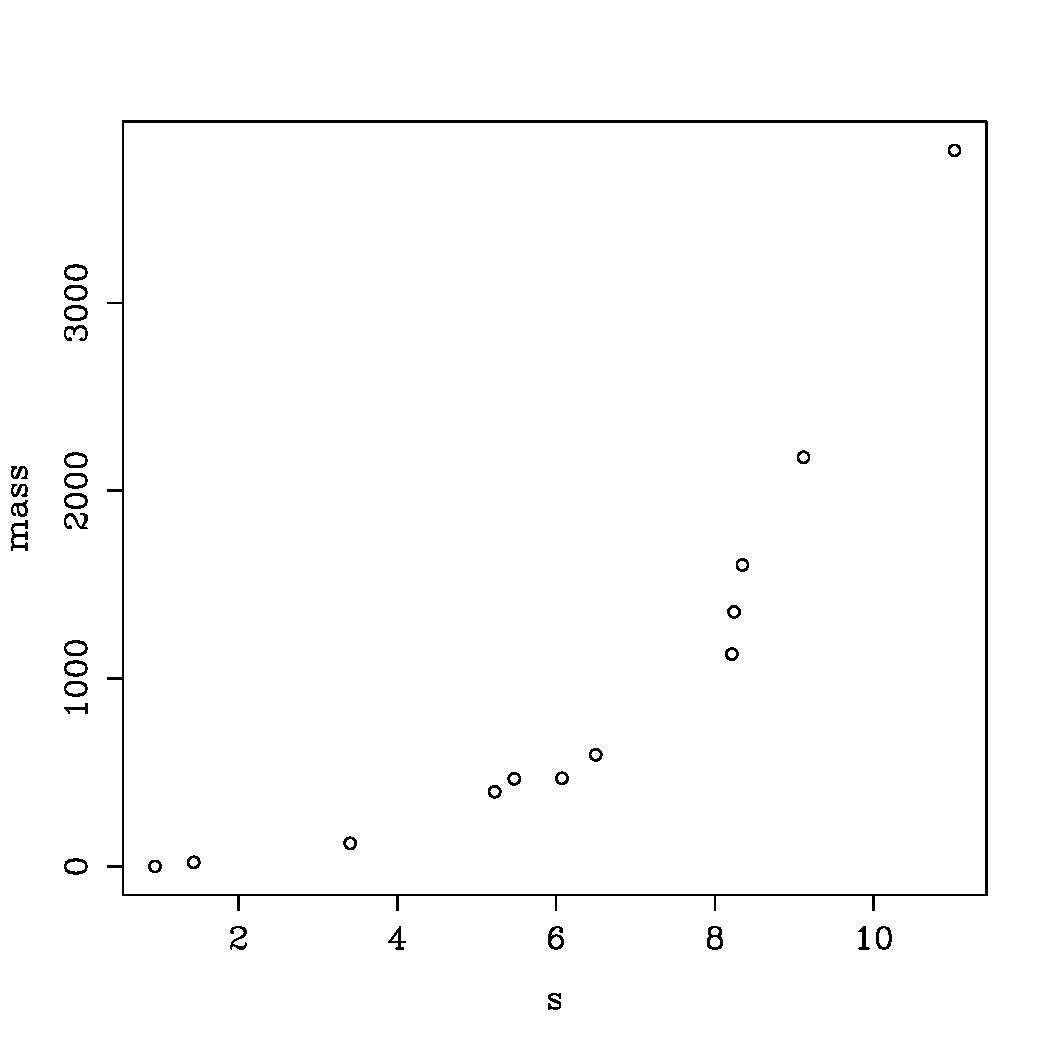
\includegraphics[width=3in]{../images/mass-v-s.pdf}
\caption{Plot of the raw data, mass vs. the length of cube side.}
\label{fig:mvss}
\end{centering}
\end{figure}

One possibility is to try plotting successive powers of $s$:  Figure~\ref{fig:mvss2} shows the mass plotted vs. the square of $s$.
\begin{figure}
\begin{centering}
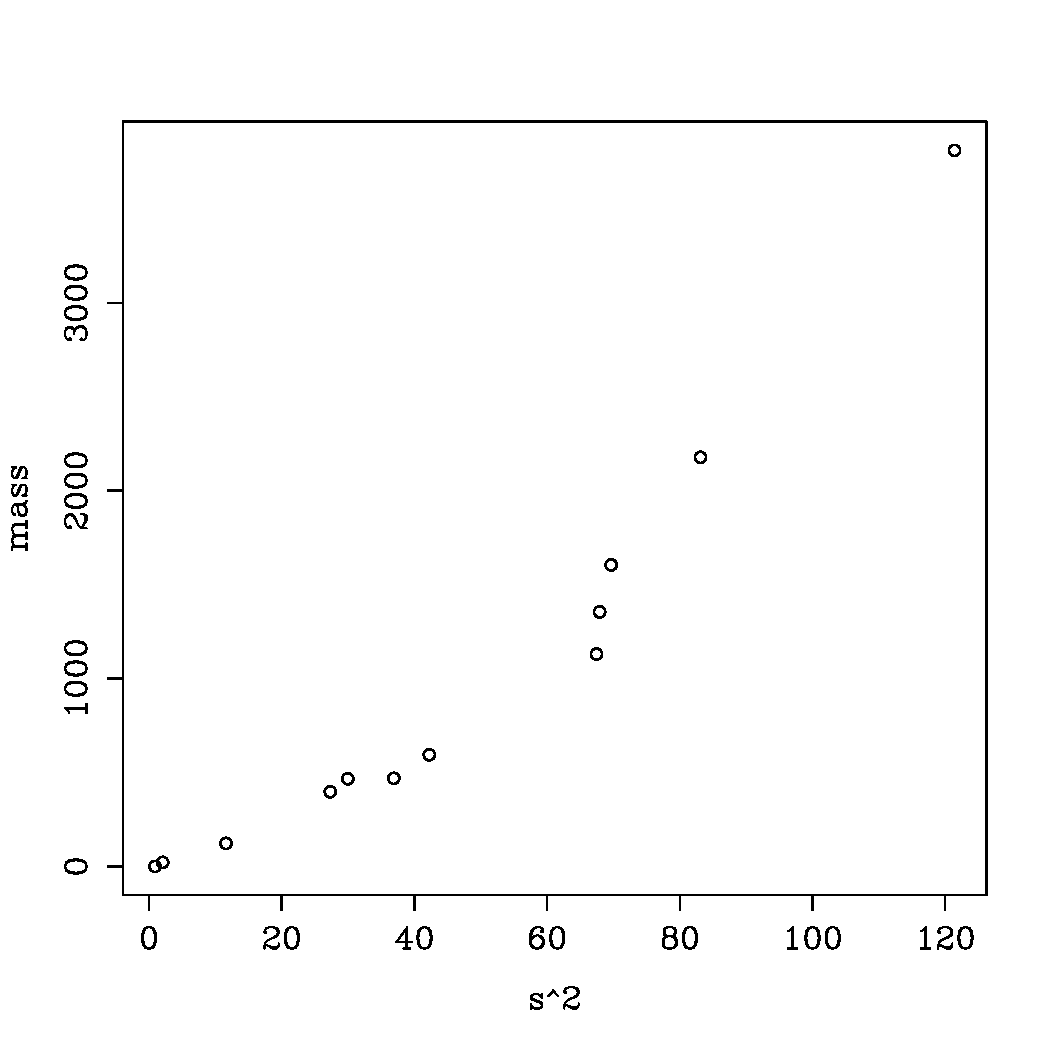
\includegraphics[width=3in]{../images/mass-v-ssq.pdf}
\caption{Plot of the data, mass vs. the length of cube side squared.}
\label{fig:mvss2}
\end{centering}
\end{figure}
Unfortunately this still doesn't work.  The data do not fall on a line, as we would have expected if the correct relationship were $m=As^2$.

We could continue like this, trying increasing powers of $s$ (and stumbling on to the correct answer next try, in this example).  But there is a better, more general technique which take advantage of properties of the log function.  A reminder:
\begin{equation}
\log(AB) = \log(A) + \log(B)
\label{eq:logprod}
\end{equation}
and
\begin{equation}
\log(A^n) = n \log(A)
\label{eq:logpow}
\end{equation}
The second of these relations is easy to show from the first, by repeatedly applying Eq.~\ref{eq:logprod} to a product of $n$ $A$s.

Now notice that if we have a function
\begin{equation}
y = A x^n
\end{equation}
and we take the log of both sides, we get
\begin{equation}
\log(y) = \log(Ax^n)
\end{equation}
and applying our above relations we get
\begin{equation}
\log(y) = n \log(x)+ \log(A)
\label{eq:loglog}
\end{equation}
which we see will result in a straight line with slope $n$ and intercept $\log(A)$ if we use $\log(x)$ on the horizontal axis (independent variable) and $\log(y)$ on the vertical axis (dependent variable).  Figure~\ref{fig:loglog} shows the result of making such a plot, and the red line is the result of a linear fit, whose slope and intercept are noted on the plot.
\begin{figure}
\begin{centering}
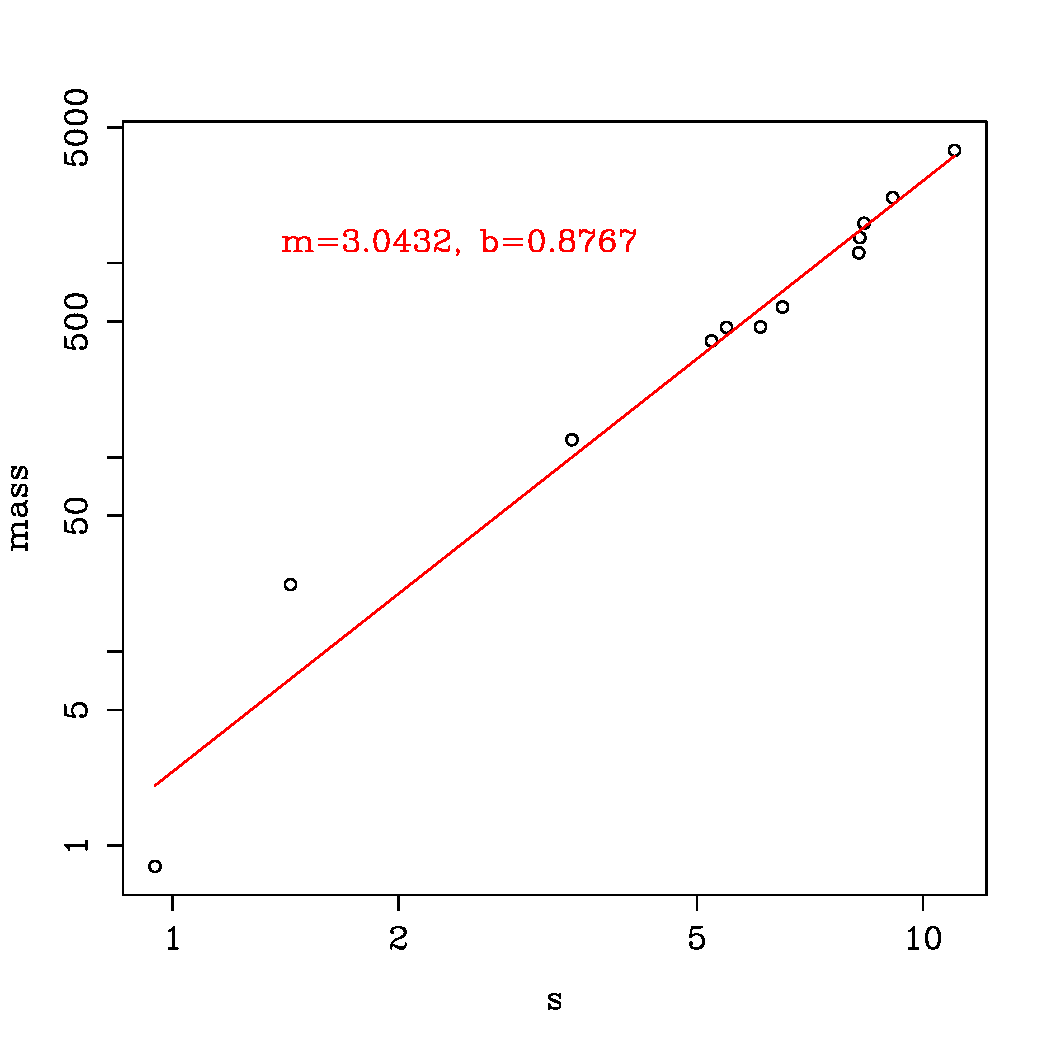
\includegraphics[width=3in]{../images/logmass-v-log-s.pdf}
\caption{Plot of the data, log(mass) vs. the log(cube side).}
\label{fig:loglog}
\end{centering}
\end{figure}
From the fitted parameters, slope = 3.04 and intercept = 0.8767, we can {\em determine} the value of the power of $s$ to be 3.04.  In other words, the mass of the object seems to depend on its volume.  From the intercept we can get a measure of the density of this material.  If we translate Eq.~\ref{eq:loglog} into its more familiar form
\begin{equation}
m = \rho V
\end{equation}
we see that $\rho = \log(A) = \log(0.8767) = 2.4 {\rm g}/{\rm cm}^3$, probably aluminum.


\end{document}
